A decision tree is a classifier that makes several sequential decisions. The outcome of that sequence determines whether a data point belongs to one class or another. The structure of a decision tree\ref{fig:DT} is defined as a set of nodes ${x_1, ... , x_n}$ with edges ${e_1, .., e_{m}}$ between them. The edges are directed and there are no cycles in the network. The tree has one root $x_1$. With each data point we start at the root. The root node is fed information about a certain feature. Each node contains a rule that allows the node to make a decision. Each decision leads to a different node, where another decision is made. This process repeats itself until one of the leaf nodes is reached\cite{safavian1991survey}. From there we can determine what class our initial data point belonged to (either class $A$, $B$ or $C$ in the figure below. 
\begin{figure}[H]
    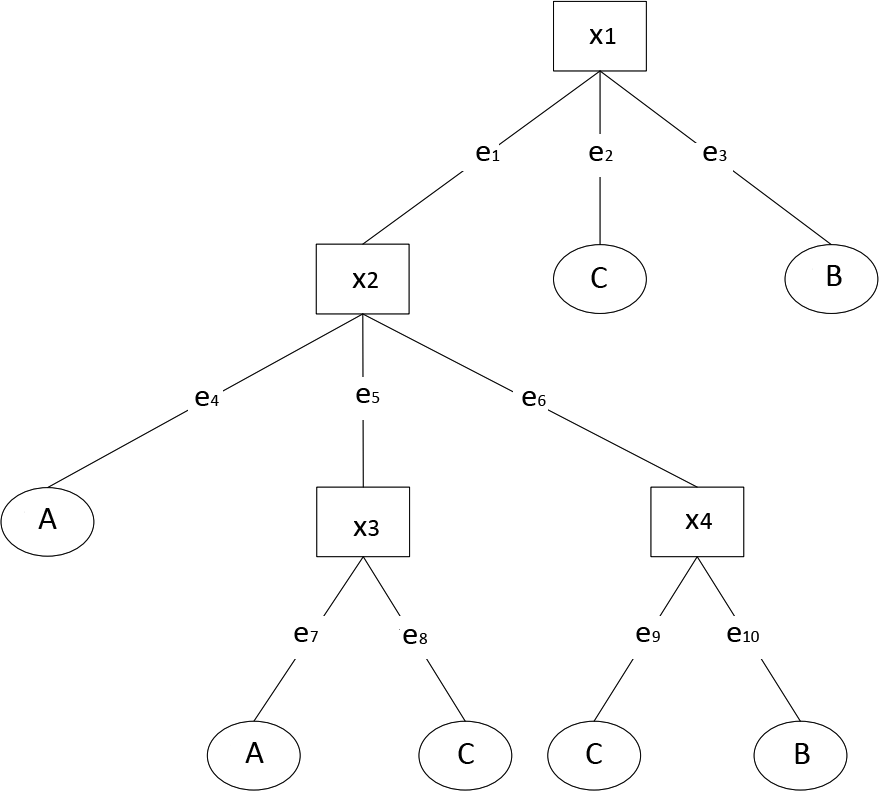
\includegraphics[width=80mm]{./img/decisiontree.png}
    \caption{Decision Tree}
    \label{fig:DT}
\end{figure}

Decision trees are generally built with a simple algorithm. Find a feature that splits up the dataset into different classes the best way. That feature will be a node. For each of the subsets that comes forth out of that division, the process is repeated until there is enough certainty that the remaining subset represents the class. This can be determined through several methods. \\

(In the first draft there will be more information on how leaf nodes are determined, how dataset can be divided into subsets, different types of decision trees and general characteristics)